\section{Depuración de la base de datos de salmones}
% TODO Corrección [14] [NO]: Parte de esta sección (procedimiento de filtrado, criterios cuantitativos y justificación) debe trasladarse al Capítulo 4 (Validación) como sección de preparación de datasets y pruebas para validar hipótesis (impacto depuración en segmentación y tracking).
En la presente memoria se expone una base de datos de salmones, la cual se origina a partir de la versión ``Salmons\_2024base'' disponible en el espacio de trabajo de WildSense en CVAT. Para optimizarla, se desarrolló un código en Python capaz de filtrar instancias irrelevantes mediante criterios de tamaño, forma y nitidez. Posteriormente, se realizaron pruebas de inspección visual con el fin de validar la capacidad de segmentación y seguimiento de los modelos entrenados con las bases de datos modificadas y determinar una versión final.

\subsection{Código de filtrado}
El código de filtrado se encarga principalmente de procesar las etiquetas de la base de datos, calculando atributos de segmentación como área, forma y nitidez. En función de estos atributos se determina si una instancia ha de ser filtrada o reasignada a otra clase. El proceso comprende tres pasos principales: la lectura de las segmentaciones, el cálculo de las métricas necesarias y, finalmente, el almacenamiento de las etiquetas depuradas en un directorio específico. Un pseudocódigo del procedimiento implementado se describe en el algoritmo~\ref{alg:filter_dataset}.

La lista completa de métricas soportadas son: \textbf{área}, \textbf{perímetro}, \textbf{relación de aspecto}, \textbf{circularidad}, \textbf{compactación}, \textbf{eccentricidad}, \textbf{elongación}, \textbf{rectangularidad} y \textbf{nitidez}. Se normalizan las métricas asumiendo una imagen de 640x640 pixeles. El código también permite filtrar las etiquetas por clase, lo que resulta útil para depurar bases de datos con múltiples clases.

Para la nitidez se utiliza una media logarítmica ponderada entre la nitidez de borde y nitidez interna. La nitidez de borde se obtiene con el promedio de la magnitud del gradiente de Sobel dentro de una banda que rodea el borde la segmentación, mientras que la nitidez interna se calcula con la varianza del filtro Laplaciano aplicado a los pixeles dentro de la segmentación.

Además, el código incluye funcionalidades para convertir bases de datos en formato CVAT (XML) a formato YOLO y, de forma inversa, exportar bases de datos YOLO en archivos ZIP aptos para su importación a CVAT. El código de filtrado se encuentra disponible de forma pública en un repositorio GitHub bajo el nombre \enquote{filter\_dataset} \cite{Lopez2025-Filter}.

\begin{algorithm}[H]
  \DontPrintSemicolon
  \SetAlgoLined
  \KwIn{Lista de polígonos (segmentaciones por imagen)}
  \KwOut{Etiquetas filtradas o reasignadas}
  % Paso 1: Leer segmentaciones
  Cargar polígonos desde la base de datos\;
  % Paso 2: Calcular características
  \ForEach{polígono $p$ en lista}{
    Calcular métricas de $p$ (área, forma, nitidez, etc.)\;
    $c \leftarrow$ \textsc{DecidirClase}(
      ¿métricas de $p$
    )\;
    \If{$c$ es clase válida}{
      Incluir o reasignar etiqueta de $p$ a clase $c$\;
    }\Else{
      Filtrar $p$\;
    }
  }
  % Paso 3: Guardar resultados
  Guardar etiquetas resultantes\;
  \caption[Algoritmo para filtrado de base de datos]{Algoritmo para filtrado de base de datos.}
  \label{alg:filter_dataset}
\end{algorithm}

\subsection{Filtrado}
En primera instancia se mejoran a mano las etiquetas dentro de la base de datos de Salmons_2024base, mejorando los contornos, combinando segmentaciones divididas en múltiples instancias o extendiendo poligonos incompletos. Luego se crea una copia local con la cual se crean las distinitas variaciones.
\begin{enumerate}% Reducir el spacing de los items
  \setlength{\itemsep}{0pt}%
  \setlength{\parskip}{0pt}%
  \setlength{\parsep}{0pt}%
  \item \textbf{SalmonesV1}: Corresponde a la base de datos original guardada localmente, sin más modificaciones que la de mejora de etiquetas.
  \item \textbf{SalmonesV2}: Se aplica un filtro basado en área, nitidez, perímetro y relación de aspecto (Código \ref{lst:snippet_filter_salmones_v2}). Luego del filtrado automático se realiza un filtrado manual, revisando la base de datos imagen por imagen, eliminando instancias borrosas y con mala visibilidad.
  \item \textbf{SalmonesV3}: Se aplica un filtro basado en solo área y perímetro (Código \ref{lst:snippet_filter_salmones_v3_v4}). También se realiza un filtrado manual a posteriori.
  \item \textbf{SalmonesV4}: Se aplica el mismo filtro que en la versión anterior, pero sin filtrado manual.
\end{enumerate}

\begin{listing}[htbp]
\caption[Criterio de filtrado usado en SalmonesV2]{\textit{Snippet} con el criterio de filtrado utilizado en la versión SalmonesV2.}
\label{lst:snippet_filter_salmones_v2}
\begin{minted}{python}
# Área pequeña
if area <= 3950:
    if nitidez <= 1.3:
      return False
    elif (nitidez >= 1.7) and (perimeter >= 300):
      return True
    else:
      return False
# Área mediana
elif 3950 < area <= 6500:   
    if nitidez <= 1.2:
      return False
    else:
      return True
# Área grande
else:
    if (nitidez < 1) and (aspect_ratio <= 0.15):
      return False
    else:
      return True
\end{minted}
\end{listing}

\begin{listing}[htbp]
\caption[Criterio de filtrado usado en SalmonesV3 y SalmonesV4]{\textit{Snippet} con el criterio de filtrado utilizado en las versiones SalmonesV3 y SalmonesV4.} 
\label{lst:snippet_filter_salmones_v3_v4}
\begin{minted}{python}
# Área pequeña
elif 1700 < area <= 4200:
    if perimeter >= 425:
      return True
    else:
      return False
# Área mediana
elif 4200 < area <= 7500:
    return True
# Área grande
else:
  return True
\end{minted}
\end{listing}

\subsubsection{Ejemplo de segmentaciones filtradas}
A continuación se muestran algunas imagenes de la base de datos Salmons_2024base y sus etiquetadas, clasificadas por área de segmentación.

\begin{figure}[h!]
\begin{center}
    % ====== Fila 1 ======
    \begin{subfigure}{0.31\textwidth}
        \centering
        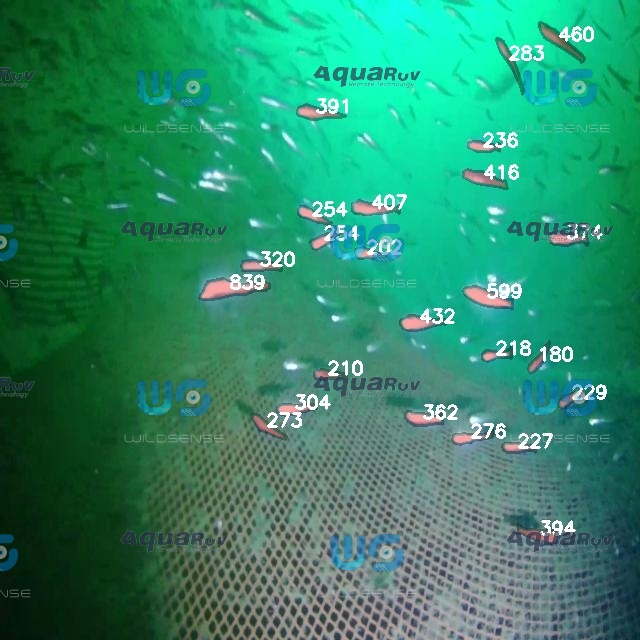
\includegraphics[width=\linewidth]{figures/filter_examples/filter1.jpg}
    \end{subfigure}
    \hfill
    \begin{subfigure}{0.31\textwidth}
        \centering
        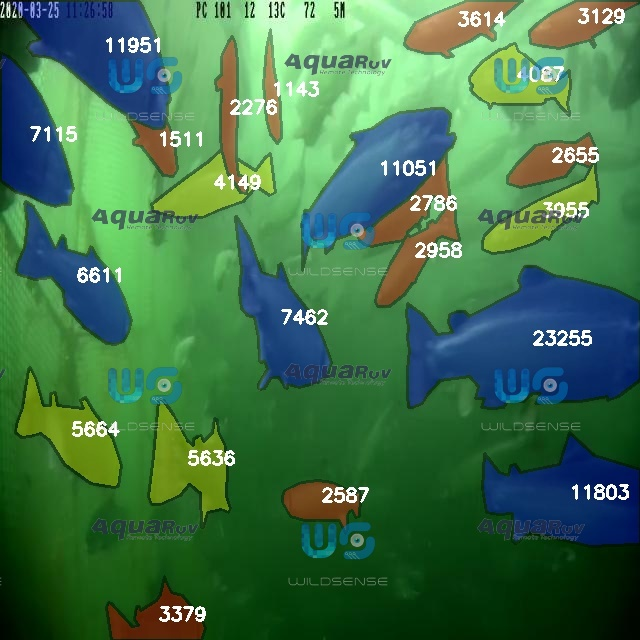
\includegraphics[width=\linewidth]{figures/filter_examples/filter2.jpg}
    \end{subfigure}
    \hfill
    \begin{subfigure}{0.31\textwidth}
        \centering
        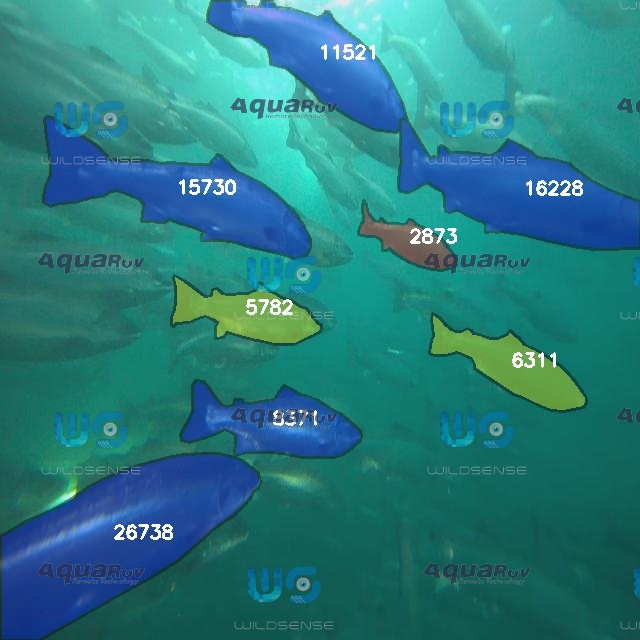
\includegraphics[width=\linewidth]{figures/filter_examples/filter3.jpg}
    \end{subfigure}
    % ====== Fila 2 ======
    \begin{subfigure}{0.31\textwidth}
        \centering
        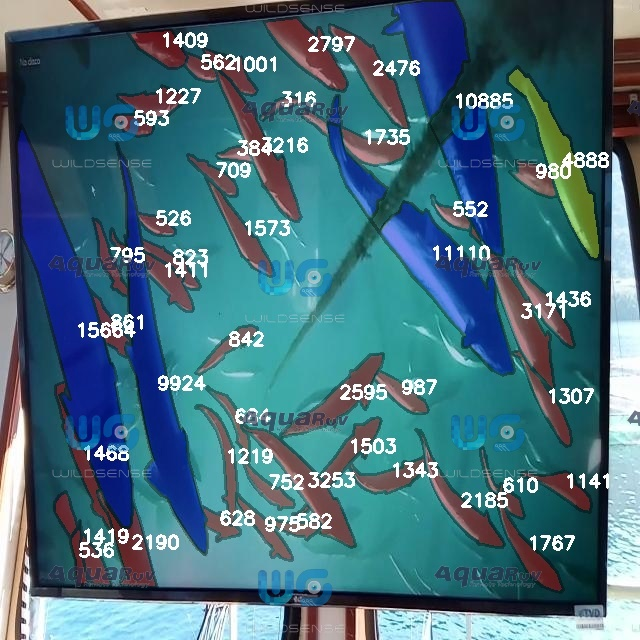
\includegraphics[width=\linewidth]{figures/filter_examples/filter4.jpg}
    \end{subfigure}
    \hfill
    \begin{subfigure}{0.31\textwidth}
        \centering
        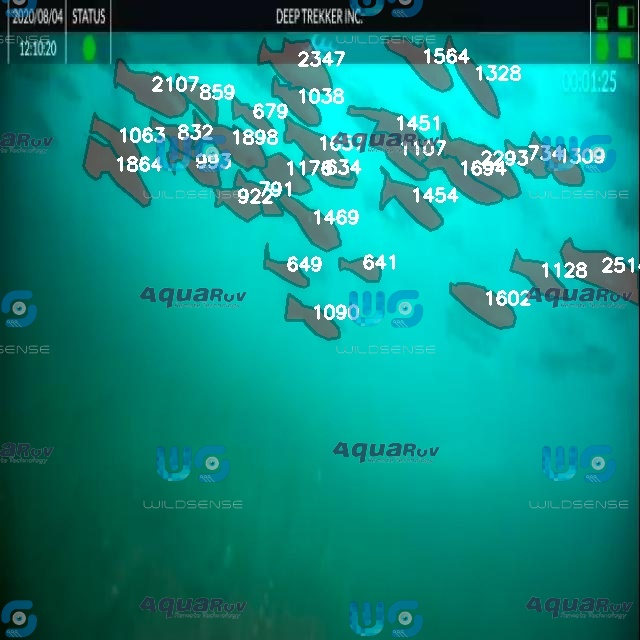
\includegraphics[width=\linewidth]{figures/filter_examples/filter5.jpg}
    \end{subfigure}
    \hfill
    \begin{subfigure}{0.31\textwidth}
        \centering
        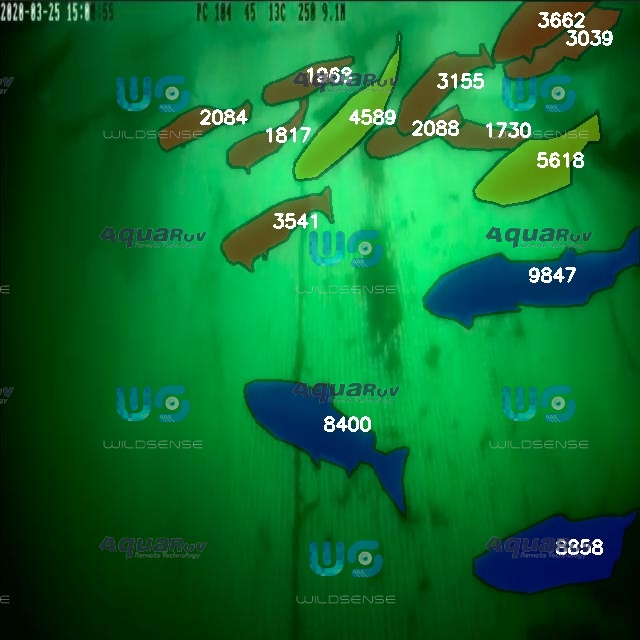
\includegraphics[width=\linewidth]{figures/filter_examples/filter6.jpg}
    \end{subfigure}
    % ====== Fila 3 ======
    \begin{subfigure}{0.31\textwidth}
        \centering
        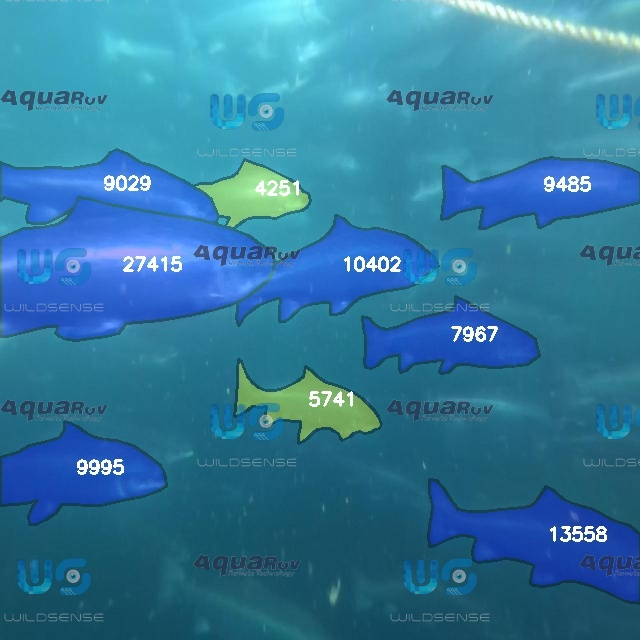
\includegraphics[width=\linewidth]{figures/filter_examples/filter7.jpg}
    \end{subfigure}
    \hfill
    \begin{subfigure}{0.31\textwidth}
        \centering
        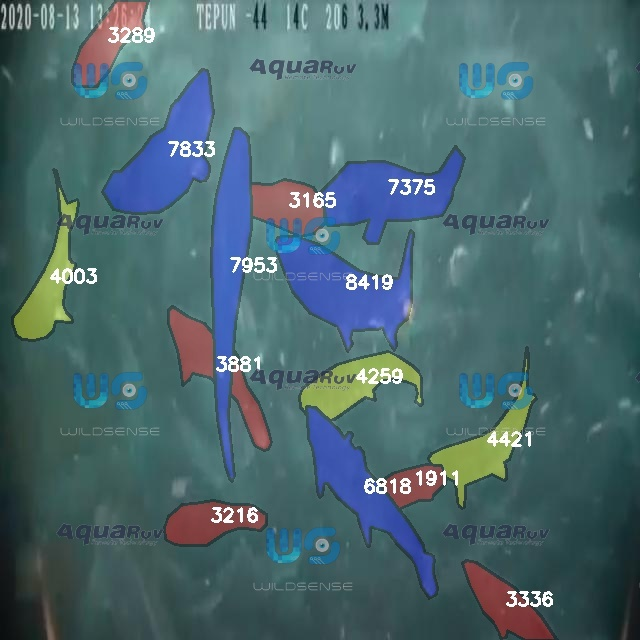
\includegraphics[width=\linewidth]{figures/filter_examples/filter8.jpg}
    \end{subfigure}
    \hfill
    \begin{subfigure}{0.31\textwidth}
        \centering
        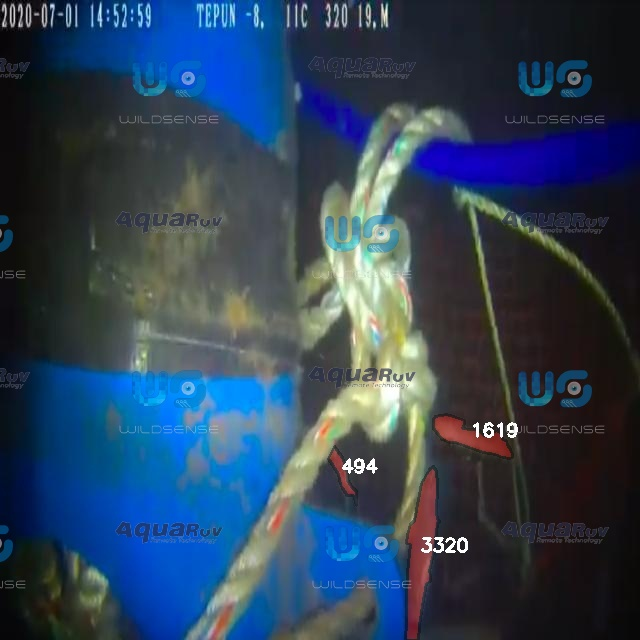
\includegraphics[width=\linewidth]{figures/filter_examples/filter9.jpg}
    \end{subfigure}
    \caption[Ejemplo de uso del código de filtrado de base de datos]{Ejemplo de uso del código de filtrado de base de datos. En rojo se muestran las segmentaciones consideradas ``pequeñas'', en amarillo las ``medianas'' y en verde las ``grandes''. El texto blanco corresponde a el área en pixeles de cada segmentación, normalizada a una imagen de 640x640 pixeles. Dependiendo del criterio de filtrado, las segmentaciones pequeñas y medianas pueden ser eliminadas o reasignadas a otra clase, igualmente se podría aplicar algún criterio de nitidez o forma.}
    \label{fig:filtered_examples}
\end{center}
\end{figure}


\subsection{Validación preliminar de bases de datos}
Como el filtrado modifica el conjunto de validación, no es posible comparar directamente el rendimiento en segmentación entre modelos entrenados con la base original y las versiones filtradas. Por ello se evalúan los \textit{datasets} usando los videos ``Seguimiento_1'' y ``Seguimiento_2''. Dado que las bases de datos de seguimiento no estaban completas, la evaluación fue cualitativa: la métrica principal fue el número de instancias detectadas (menos es mejor al indicar menor ``parpadeo'') y se inspeccionó visualmente la calidad de las segmentaciones. Se utilizaron modelos YOLOv8l-seg para las pruebas, tanto en formato PyTorch como TensorRT.

\begin{table}[htbp]
\centering
\caption[Evaluación entre distintas versiones de la base de datos de salmones]{Comparación del número de instancias seguidas por modelos YOLOv8l de segmentación entrenados con diferentes versiones de la base de datos de salmones.}
\label{tab:seguimientos_versiones_dataset}
\begin{tabular}{|c|r|r|c|}
\hline
\textbf{Dataset} & \multicolumn{1}{c|}{\textbf{Seguimiento\_1}} & \multicolumn{1}{c|}{\textbf{Seguimiento\_2}} & \textbf{Formato} \\ \hline
\multirow{2}{*}{SalmonesV1} & 323.0 & 252.0 & Pytorch \\ \cline{2-4} 
 & 188.0 & 185.5 & TensorRT \\ \hline
\multirow{2}{*}{SalmonesV2} & 94.5 & 263.5 & Pytorch \\ \cline{2-4} 
 & 51.5 & 94.0 & TensorRT \\ \hline
\multirow{2}{*}{SalmonesV3} & 106.5 & 176.5 & Pytorch \\ \cline{2-4} 
 & 69.0 & 106.0 & TensorRT \\ \hline
\multirow{2}{*}{SalmonesV4} & 99.0 & 149.0 & Pytorch \\ \cline{2-4} 
 & 58.0 & 78.5 & TensorRT \\ \hline
\end{tabular}
\end{table}

Se selecciona SalmonesV4 por ofrecer una disminución notable en el número de instancias detectadas junto con una buena calidad de segmentación. Al prescindir de filtrado manual, esta versión es además menos sesgada y, por tanto, más robusta y generalizable frente a los criterios de tamaño considerados en el proyecto.

\subsection{Evolución}
Al depurar la base de datos se eliminan numerosas etiquetas sin retirar las imágenes, con el fin de mejorar la calidad de las segmentaciones y el rendimiento en detección. Una consecuencia de esta limpieza es un aumento en la proporción de imágenes de fondo; aunque aportan contexto valioso sobre escenas sin salmones de interés, también puede introducir ruido irrelevante que, en exceso, perjudique la capacidad de generalización del modelo entrenado.

\begin{table}[htbp]
\centering
\caption[Composición de las bases de datos de salmones filtradas]{Composición de las bases de datos de salmones elaboradas, sin filtrado manual.}
\label{tab:salmones_evolution}
\begin{tabular}{|c|c|c|c|c|}
\hline
\textbf{Dataset} & \textbf{Tarea} & \textbf{Num. imgs.} & \textbf{Num. segm.} & \textbf{Img. fondo} \\ \hline
\multirow{4}{*}{SalmonesV1} & Train & 903 & 4517 & 356 \\ \cline{2-5} 
 & Validation & 56 & 526 & 0 \\ \cline{2-5} 
 & Testing & 2 & 16 & 0 \\ \cline{2-5} 
 & \textbf{Total} & \textbf{961} & \textbf{5059} & \textbf{356} \\ \hline
\multirow{4}{*}{SalmonesV2} & Train & 903 & 1686 & 544 \\ \cline{2-5} 
 & Validation & 56 & 81 & 26 \\ \cline{2-5} 
 & Testing & 2 & 13 & 0 \\ \cline{2-5} 
 & \textbf{Total} & \textbf{961} & \textbf{1780} & \textbf{570} \\ \hline
\multirow{4}{*}{SalmonesV3} & Train & 903 & 1793 & 524 \\ \cline{2-5} 
 & Validation & 56 & 120 & 26 \\ \cline{2-5} 
 & Testing & 2 & 15 & 0 \\ \cline{2-5} 
 & \textbf{Total} & \textbf{961} & \textbf{1928} & \textbf{550} \\ \hline
\multirow{4}{*}{SalmonesV4} & Train & 903 & 1793 & 524 \\ \cline{2-5} 
 & Validation & 56 & 120 & 26 \\ \cline{2-5} 
 & Testing & 2 & 15 & 0 \\ \cline{2-5} 
 & \textbf{Total} & \textbf{961} & \textbf{1928} & \textbf{550} \\ \hline
\end{tabular}
\end{table}

\subsection{Elaboración final de la base de datos de salmones}
Como se explica en la sección \ref{sec:datasets}, a la base de datos filtrada ``SalmonesV4'' se le incluyeron imágenes y etiquetas adicionales pertenecientes a los videos ``Seguimiento_1'' y ``Seguimiento_2''. Las etiquetas fueron revisadas manualmente, se removieron aquellas instancias que no cumplían con los criterios de calidad establecidos y se incluyeron cientos más para secciones de los videos que estaban sin etiquetar. Se combinaron las imágenes y etiquetas de forma aleatoria con la siguiente distribución según la tarea: 65\% para entrenamiento, 30\% en validación y 5\% para pruebas. El resultado final es la base de datos ``Salmons'' descrita anteriormente (tabla \ref{tab:datasets_combined}).
